\section{Software process improvement and capability determination}\label{app:spice}
Lo standard internazionale ISO/IEC 15504 definisce il modello SPICE per la valutazione dei processi di produzione software.\\
Il modello SPICE valuta i processi secondo diversi aspetti e ne determina le capacità.
Per ogni processo è stabilito il livello di maturità in base ai suoi attributi secondo una scala di livelli predefinita:
\begin{enumerate}
	\setcounter{enumi}{-1}
	\item \textbf{Incomplete process}: le performance del processo, come i suoi risultati, sono incompleti.
	\item \textbf{Performed process}: i processi sono eseguiti intuitivamente per raggiungere dei risultati. Attributi: 
		\begin{itemize}
			\item \textbf{process performance}: gli obiettivi sono raggiunti trasformando input identificabili in output identificabili.
		\end{itemize}
	\item \textbf{Managed process}: i processi e i prodotti dei processi sono gestiti e le responsabilità sono definite. Attributi:
		\begin{itemize}
			\item \textbf{performance management}: il prodotto è coerente con gli obiettivi fissati;
			\item \textbf{work product management}: il prodotto è documentato, controllato e verificato. 
		\end{itemize}
	\item \textbf{Established process}: il processo è definito o estrapolato da uno standard. Attributi:
		\begin{itemize}
			\item \textbf{process definition}: l'esecuzione del processo si basa su standard;
			\item \textbf{process deployment}: il processo usufruisce delle risorse in modo efficace.
		\end{itemize}
	\item \textbf{Predictable process}: sono definite metriche per le performance di processo e per i risultati prodotti. Attributi:
		\begin{itemize}
			\item \textbf{process measurement}: vengono utilizzate le misure, le metriche e gli obiettivi per garantire il raggiungimento dei traguardi;
			\item \textbf{process control}: vengono utilizzate misure e metriche per controllare processi e prodotti, al fine di effettuare correzioni migliorative.
		\end{itemize}
	\item \textbf{Optimizing process}: misure quantitative sono utilizzate per l'analisi di performance di processo e dei suoi risultati per attuarne il continuo miglioramento. Attributi:
		\begin{itemize}
			\item \textbf{process innovation}: applicazione di approcci innovativi;
			\item \textbf{process optimization}: ottimizzazione controllata e misurata di processo.
		\end{itemize}
\end{enumerate}
Gli attributi di processo sono stimati in punti percentuale secondo quattro livelli: 
\begin{itemize}
	\item 0-15\% non compiuto (N);
	\item 15-50\% parzialmente compiuto (P);
	\item 50-85\% largamente compiuto (L);
	\item 85-100\% completamente compiuto (C).
\end{itemize}
\begin{figure}[H]
	\centering
	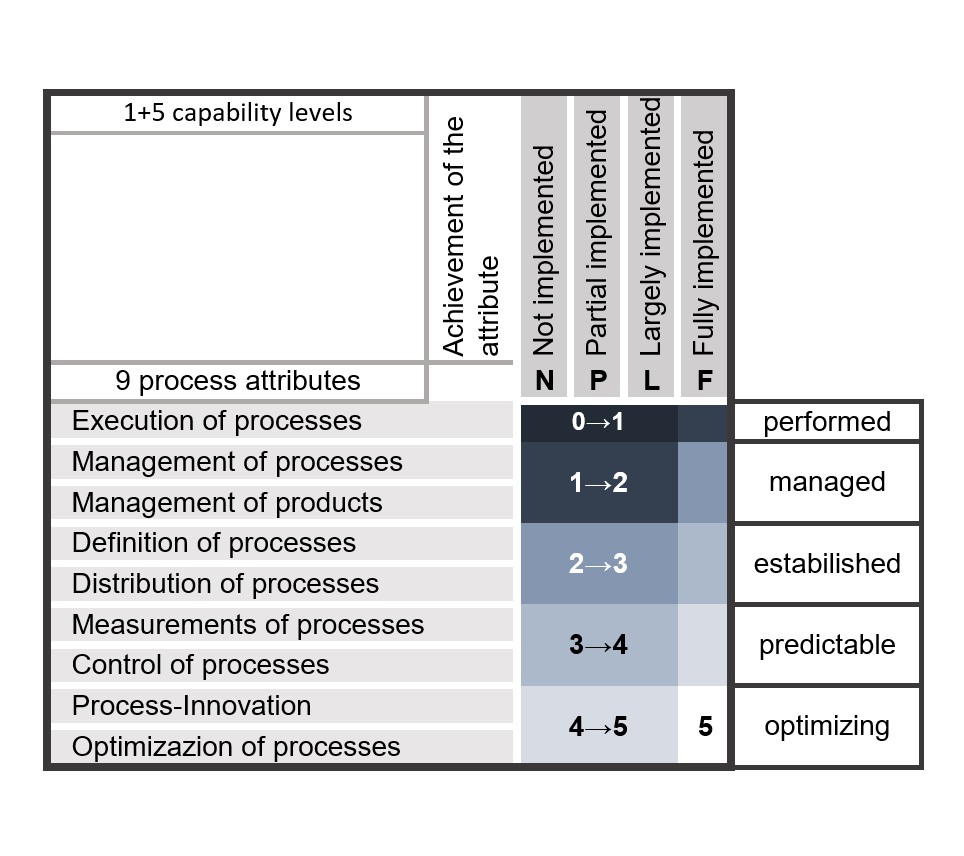
\includegraphics[width=13cm]{spice.png}
	\caption{Valutazioni del modello \glossario{ISO}/\glossario{IEC} 15504}
\end{figure}
